\documentclass[11pt]{article} 
\usepackage[utf8]{inputenc} 
\usepackage{geometry} 
\geometry{a4paper} 
\usepackage{graphicx}





\title{Big Data Analytics Project : Dataset Adult from UCI }
\author{Mohammed Meftah, Raunaq Paul and Binxiang Xiang}
\date{$16^{th}$ January 2017}

\begin{document}
\maketitle
\tableofcontents

\newpage
\section{Introduction}
For this project, we have decided to work on the dataset Adult from UCI. This is a classification dataset with two classes, as we have to understand and predict whether a person earns less or more than 50k dollars a year, according to the provided features. Section 2 describes in details the used dataset Adult. Section 3 highlights how we first processed data. Section 4 shows some statistical analysis on the dataset. Section 5 presents the methodology and the performances of different algorithms (list of tried algo to add) on the prediction of our target variable. 

\section{Dataset description}
The raw dataset has 48842 rows and 15 columns including the target variable. This data is originally from the american census bureau and shoulb be representative of the american population. This dataset is mixing continuous variables and discrete variables as follows : 

\begin{description}\itemsep0.5pt
\item[age] : continuous, age of the individual.
\item[fnlwgt] : continuous, the number of people the observation should represent, not useful for us.
\item[workclass] : discrete, 8 categories representing the type of the employer of the individual ( Private, Federal-gov, Never-worked ...).
\item[education] : discrete, 16 categories representing the highest level of education achieved by the individual (Bachelors, Masters, Doctorate, Highschool grad ... ).
\item[educationnum] : continuous, number of years of education.
\item[mstatus] : discrete, 7 categories representing the marital status of the individual(Divorced, Never-married, Separated ... ).
\item[occupation] : discrete, 14 categories representing the occupation of the individual (Tech-support, Sales, Exec-managerial, Other-service ...).
\item[relationship] : discrete, 6 categories representing the relationship of the individual, we don't know with who so this variable is not very clear (Wife, Husband,Own-child ...).
\item[race] : discrete, 5 categories representing the race of the individual (White, Asian-Pac-Islander, Black, Amer-Indian-Eskimo and Other).
\item[sex] : discrete, sex of the individual (Female or Male).
\item[capitalgain] : continuous, represents the recorded capital gains.
\item[capitalloss] : continuous, represents the recorded capital losses.
\item[hoursperweek] : continuous, represents the number of hours worked per week.
\item[nativecountry] : discrete, 41 categories representing the country of origin of the individual.
\item[target] : discrete, variable to predict, 2 classes ($<= 50k\$$ or $>50k\$$).
\end{description}
For the next sections, these names will be used to refer to the corresponding variable.
\section{Data processing}
In this section, we explain the different steps of processing we did on our raw dataset.
\subsection{Basic processing : }
We did perform some basic processing as a first step : 
\begin{itemize}
\item Remove the variable \emph{fnlwgt}, as it is not an information on the individual.
\item Remove the variable \emph{educationnum}, as it contains the same information as the variable \emph{education} and we would prefer to work with a discrete variable.
\item Transform the target variable into binary values,  0 if $<=50k\$$ 1 if $>50k\$$.
\item Remove rows with missing values, indeed variables \emph{workclass}, \emph{occupation} and \emph{nativecountry} don't always have values. It represents 3620 rows.
\item Scale continuous variables : \emph{capitalgain,capitalloss and hoursperweek}
\end{itemize}
After these steps, the new dataset has 45222 rows. And 24.8\% of the observations are in the class 1 and 75.2\% are in the class 0.
\subsection{Advanced processing :}
As the discrete variable \emph{nativecountry} contains 41 categories where the main one (United States) represents 91.3\% of the total, we have decided to group countries together into bigger categories. We don't change United-States, Canada, Japan, China, India , Iran and Mexico. The changes are the following :

\begin{center}

\begin{tabular}{|c|c|}
\hline
New value & Old values concerned \\
\hline
WEurope & England, France, Germany, Holand-Netherlands,\\
& Ireland, Italy, Portugal, Scotland\\
\hline
EEurope & Greece, Hungary, South, Yugoslavia\\
\hline
SEAsia & Cambodia, Laos, Philippines, Thailand, Vietnam\\
\hline
 LatAmerica & Columbia, Cuba, Dominican-Republic, Ecuador, El-Salvador, \\
&Guatemala, Haiti, Honduras, Jamaica, Nicaragua, \\
&Outlying-US(Guam-USVI-etc), Peru, Puerto-Rico, Trinadad\&Tobago \\
\hline
China & HongKong, Taiwan \\
\hline
\end{tabular}
\end{center}
After the transformation, our \emph{nativecountry} variable has now 11 different values against 41 before. Of course, we lost some information but it shoud not be so significant as we regroup countries from same area and with similar economic situation.



\section{Analysis}
After the processing part, we can start to look at data and make some analysis by variable and by class. We separated the study whether the variables are numeric or categorical.

\subsection{Numerical features}
We first study the correlation of numerical variables with the target. We thus made the following corrplot :

\begin{figure}[!h]
	\centering
	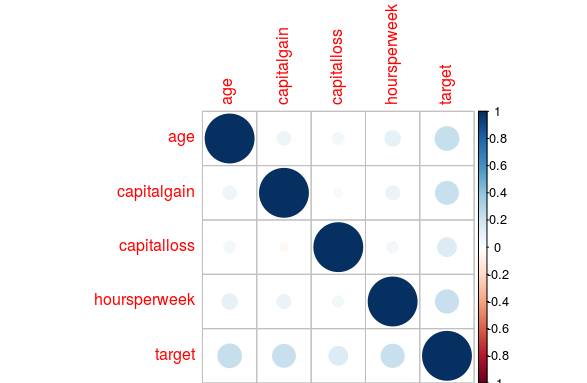
\includegraphics[width=.6\textwidth]{images/plot_corr.png}
\end{figure}
It shows that all the numerical variables are correlated positively with the target. However the correlation values remains low with the best score for (age, target) around 0.3. So for a first model, maybe it is not of paramount importance to include such variables.

\subsection{Categorical features}
We cannot define a correlation properly with categorical variables. We choose to look at the distribution of the target within the categorical variables and test their independance ($\chi$-squared test) with the target in order to have an idea of each possible contribution.

\begin{center}
\begin{tabular}{|c|c|c|}
\hline
Feature & $\chi$-square & $p$-value \\
\hline
race & 452.3 & $<$2.2e-16\\
workclass & 1207.3 & $<$2.2e-16\\
mstatus & 9109.2 & $<$2.2e-16\\
sex & 2104.1 & $<$2.2e-16\\
nativecountry & 379.36 & $<$2.2e-16 \\
education & 6000 & $<$2e-16\\
\hline
\end{tabular}
\end{center}

The $\chi$-square tests are very concluding so we are confident to reject the null hypothesis and consider that each of these categorical variables are non-independant with the target, it means that they are correlated. The very low p-values pinpoint also this high correlation. We should see some pattern by looking at the target distribution for each unique element of each feature.


\begin{figure}[!h]
	\centering
	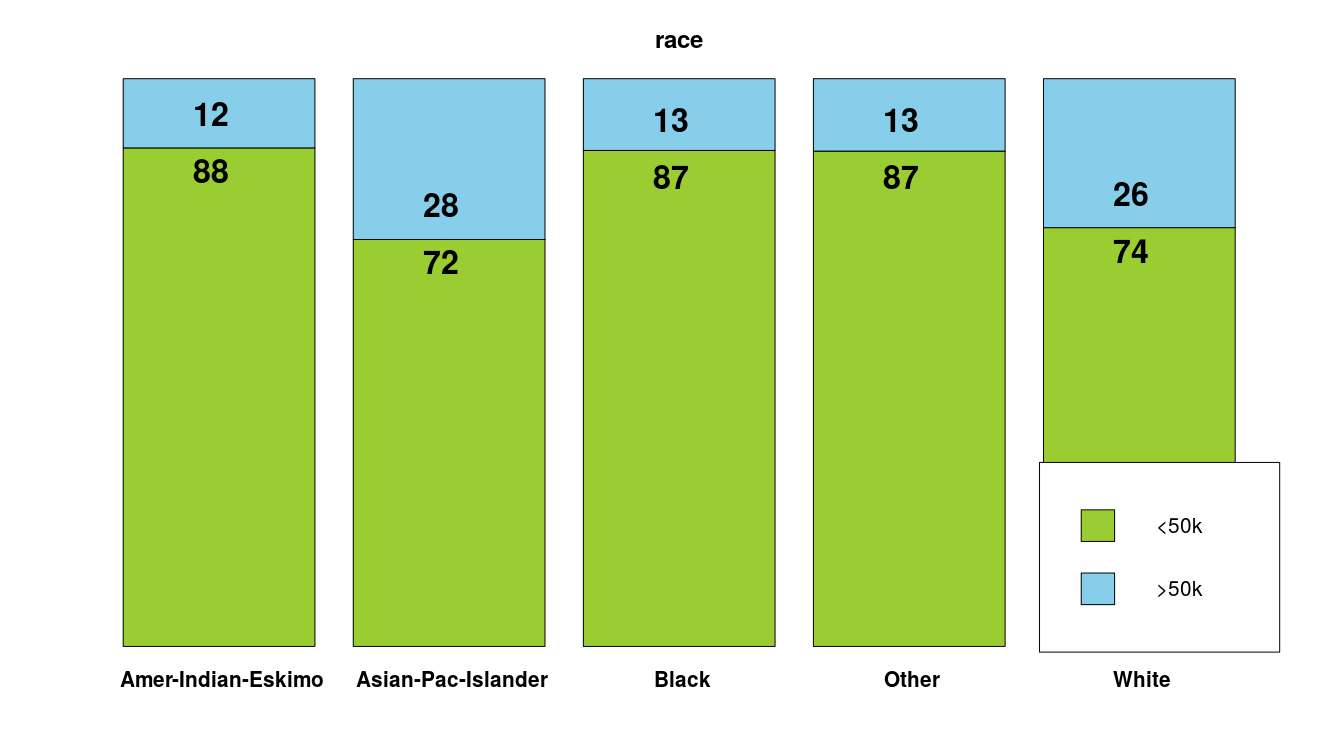
\includegraphics[width=.5\textwidth]{images/plot_race.png}%
	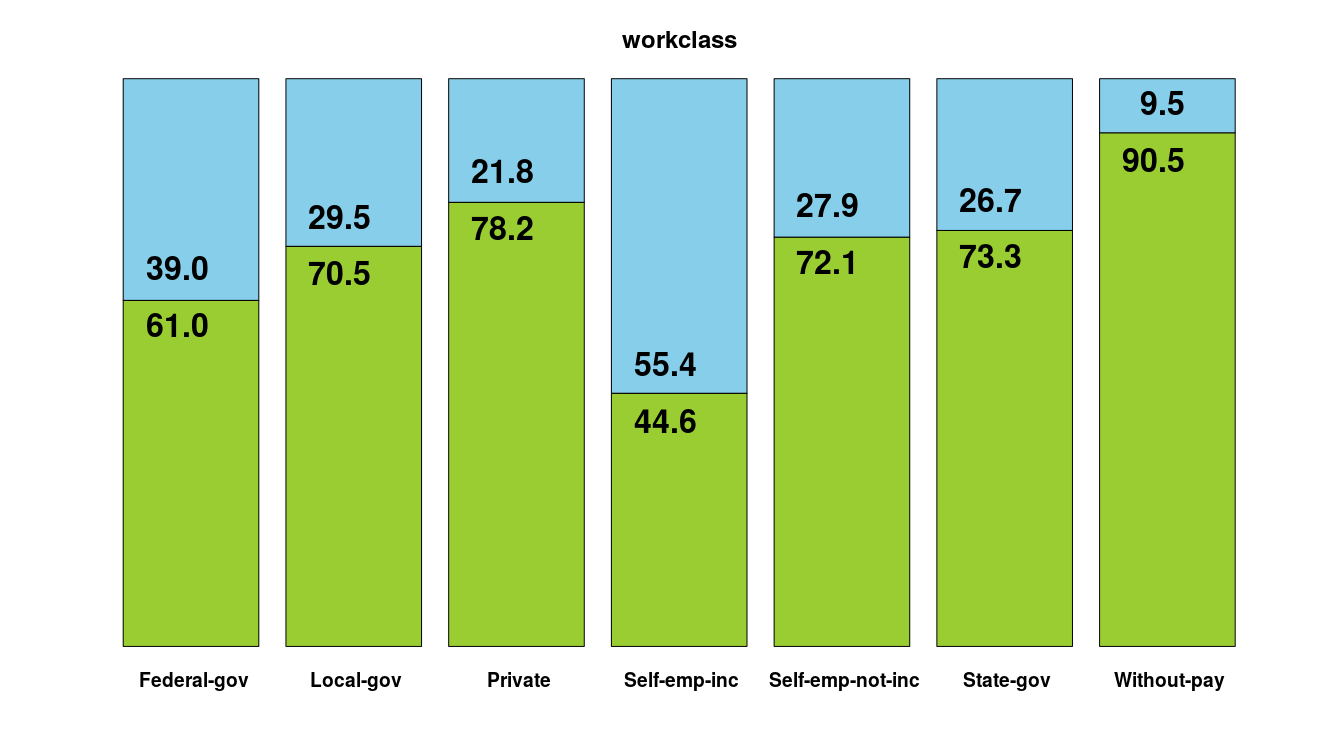
\includegraphics[width=.5\textwidth]{images/plot_workclass.png}
	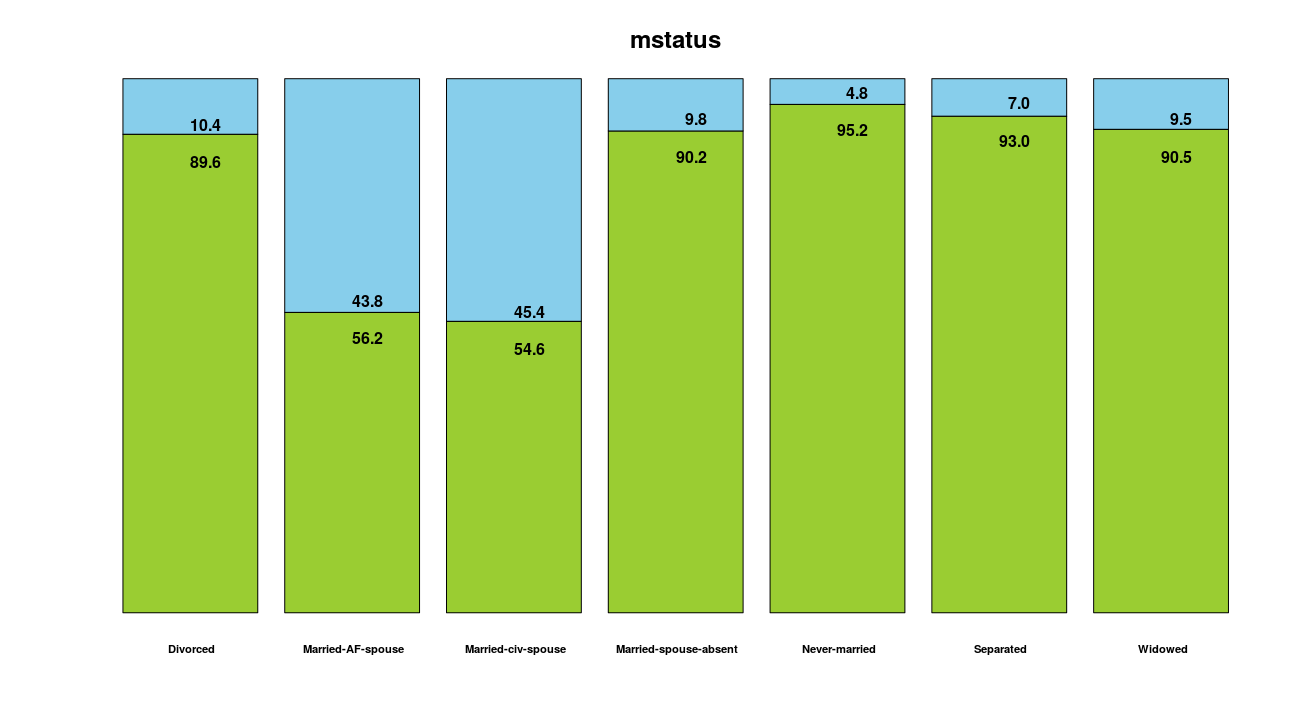
\includegraphics[width=.5\textwidth]{images/plot_mstatus.png}%
	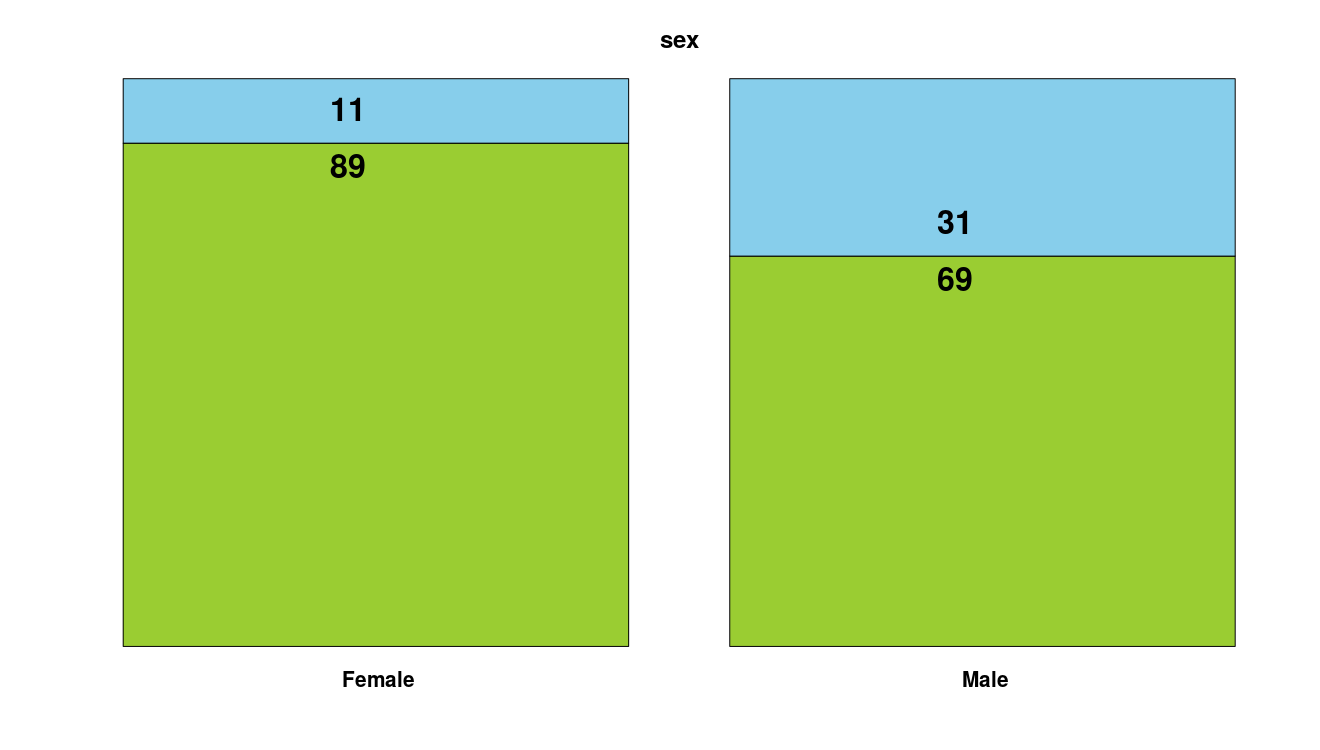
\includegraphics[width=.5\textwidth]{images/plot_sex.png}
	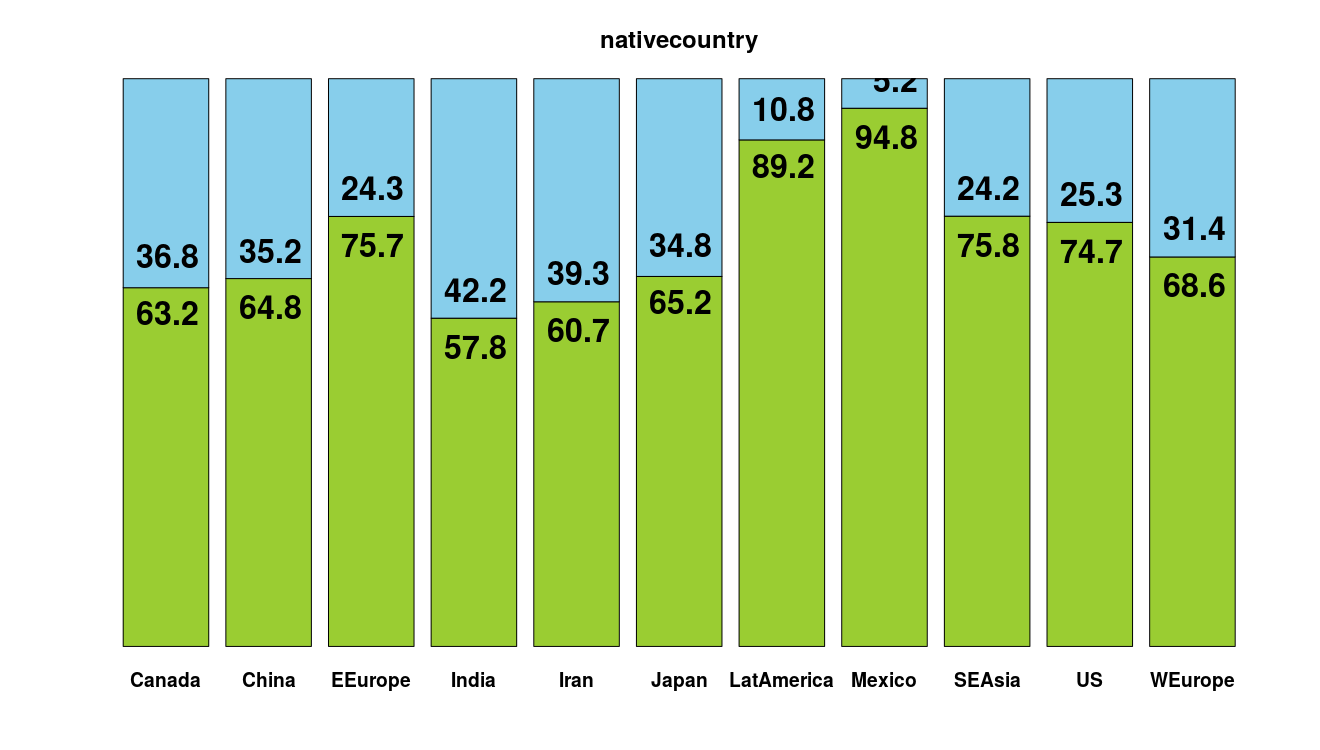
\includegraphics[width=.5\textwidth]{images/plot_nativecountry.png}%
	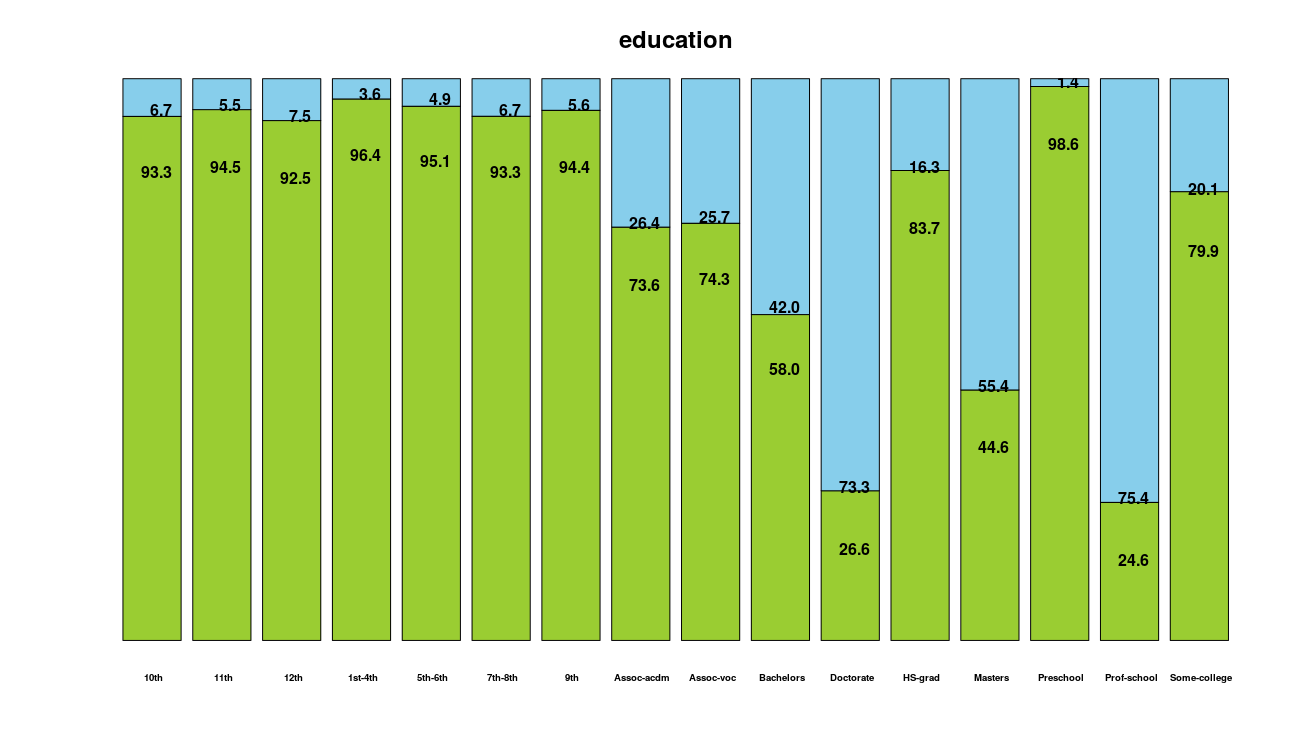
\includegraphics[width=.5\textwidth]{images/plot_education.png}
\end{figure}

As we clearly see, for almost all this categorical features, the distribution of the target is not homogenous within the feature labels. It should enable us to make better predictions with these features as a basis. And some of the distributions are confirming some common knowledge. For example, in proportion more men (31\%) are in the $>50k\$$ category than women (11\%) or people with PhD (73\%) are more prone to be in the class 1 than people with master degree (53.4\%) or bachelor degree (42\%).
We can see some other interesting insights too, for example, divorced people (10.4\%) are less prone to be in the class 1 than married people ($\approx$44\%). In terms of proportion, more Asian people (28\%) are earning more than 50k\$ than other minorities(12-13\%) and they even outreach white people. 
\section{Methodology and results}
\subsection{Methodology}
In this section, we'll describe the procedure in order to compare different algorithms we have chosen on our dataset. These algorithms are Logistic Regression (LogReg), Bagging, Random Forest (RF) and K-Nearest Neighbours. 
The difficulty here is that our dataset is mixing continuous and discrete variables. For the first three methods, it wasn't an issue as they deal easily with a mix of continuous and discrete variables. But for K-Nearest Neighbours, we had to transform the discrete variables before applying the model. We'll describe very precisely what we did for KNN and we'll see that the performances are surprisingly very good for KNN. 


To compare the different algorithms, we perform the following procedure :

\begin{enumerate}
\item Find the best hyperparameters for our model by Cross Validation
\item Split randomly dataset into train and test sets, 70\% in the train set and 30\% in
test set.
\item Train the algorithm on the train set
\item Predict values on the test set
\item Save the prediction error with accuracy measure
\item Repeat 20 times steps 2 to 5
\item Do steps 1 to 6 for each method (algorithm)

\end{enumerate}
\newpage
\subsection{Results}
\subsubsection{Logistic Regression, RF and Bagging}
We'll not detail the hyperparameters selection for Random Forest and Bagging. Here are the results of Logistic Regression, optimized Random Forest and optimized Bagging : 

\begin{figure}[!h]
\begin{center}
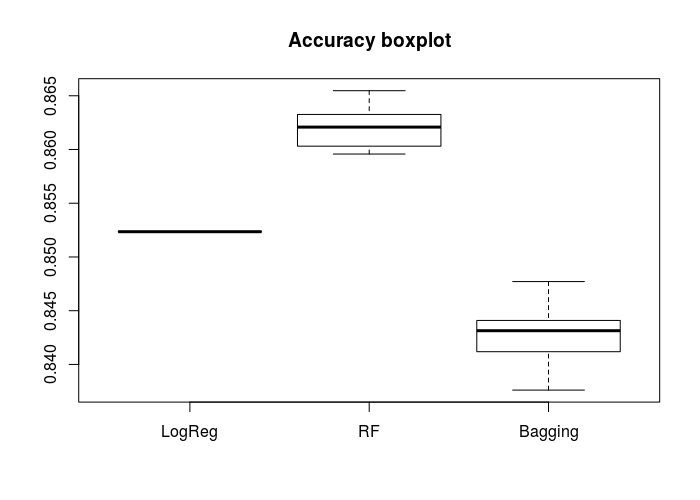
\includegraphics[scale=0.8]{images/accuracy_boxplot.png}

\end{center}
\caption{20 runs Accuracy boxplot for LogReg, RF and Bagging}
\end{figure}

Among these three methods, the best performing one is Random Forest with an average accuracy of \textbf{0.862}. Furthermore, we can notice that Logistic regression is very robust. The performances are very stable even though the train and test set are not the same.

\subsubsection{K-Nearest Neighbours}

As we said before, we can't directly apply KNN on our dataset. We need to transform our discrete variables into numeric variables, on which KNN will be able to build a metric. Besides, we can't just create a correspondence table. Indeed, if we choose to code the n values/categories of a discrete variable by a set of n integers, we'll introduce some order relationships. For instance, for the variable race, if we code 'White' by 1, 'Black' by 2 , 'Asian' by 3 and so on, we will have relationships like 'Black' $>$ ''White' or 'Asian' = 3*'White', which are not true here.  

A common method to solve this problem is to transform discrete variables into dummy variables. That's what we did on our dataset, we transformed each discrete variable into dummy variables. At the end, we obtained 72 features excluding the target variable. The number of features is too big, we need to perform dimension reduction either because of the curse of dimensionality or because of the computational time. However, the screeplot (Fig. 2) of a PCA on our dataset did not give us something very remarkable so we decided to choose the number of features to keep by looking at the performances. 

\begin{figure}[!h]
\begin{center}
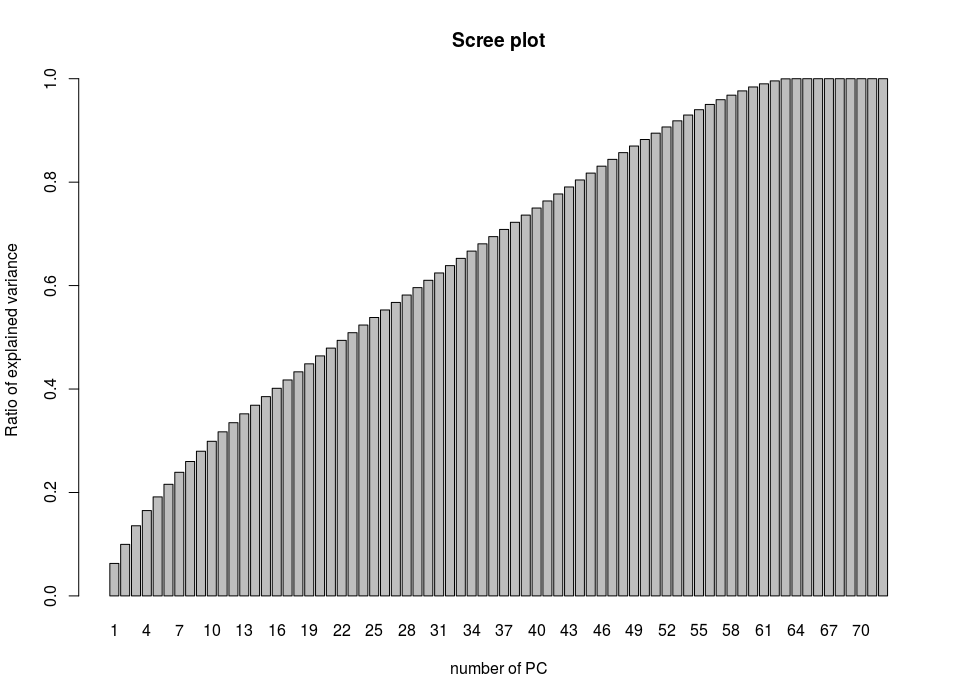
\includegraphics[scale=0.6]{images/screeplot.png}

\end{center}
\caption{Screeplot for our dataset}
\end{figure}
\newpage
Figure 3 presents the boxplot of a 3-NN for different number of kept features (after 5 runs): 

\begin{figure}[!h]
\begin{center}
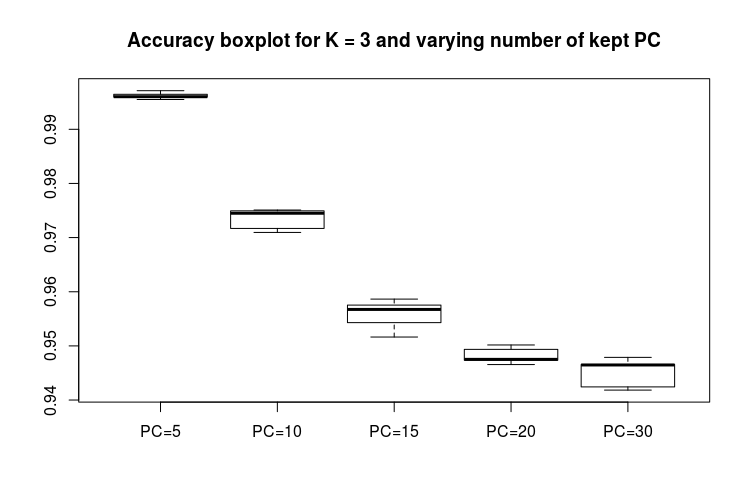
\includegraphics[scale=0.8]{images/KNN_PCA.png}

\end{center}
\caption{Accuracy boxplot for 3 NN and different number of principal components}
\end{figure}

So, we can see that if we project our data into a space of dimension 5 with PCA, the performances are astonishingly good ( average accuracy of even if the corresponding explained variance is around 20\%. Without doubt, we decide to keep the 5 first principal components in order to project our data. 
\newpage
So with this parameter fixed, figure 4 presents performances when we vary the parameter K of number of nearest neighbours. 

\begin{figure}[h]
\begin{center}
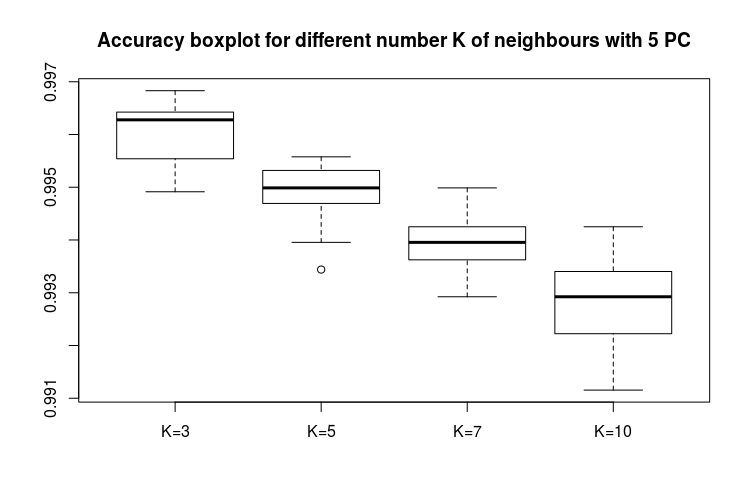
\includegraphics[scale=0.7]{images/Knn_accuracy.png}

\end{center}
\caption{Accuracy boxplot for varying number of Nearest Neighbours and 5 PC}
\end{figure}



So, performances are the best for K=3. We have an average accuracy of \textbf{0.996}. This method outperformed Logistic Regression, Random Forest and Bagging.  But the problem is that we can't really explain which features were valuable as we performed PCA on our dataset.



\section{Conclusion}







\end{document}
